\documentclass[11pt]{report}
\usepackage[margin=2cm]{geometry}
\usepackage[fleqn]{amsmath}
\usepackage{nccmath}
\usepackage{alltt}
\usepackage{sectsty}
\usepackage{titlesec}
\newcommand{\ts}{\textsuperscript}
\usepackage{graphicx}
\graphicspath{ {../images/} }
\usepackage{subfig}
\usepackage[hidelinks]{hyperref}
\newcommand{\linespace}{\vspace{0.3cm}\noindent}
\renewcommand{\bibname}{References}
\usepackage{multirow}

\titlespacing*{\section}{0pt}{0.8\baselineskip}{0.2\baselineskip}

\begin{document}

\begin{titlepage}
    \begin{center}
        \vspace*{1cm}
        
        \textbf{CO3093 COURSEWORK 2 - Report}
        
        \vspace{0.5cm}
		Big Data \& Predictive Analytics - Classification \& Clustering
        
        \vspace{1.5cm}
        
        \textbf{Ihtasham Chaudhry}
        
        \vfill
        
        \vspace{0.8cm}
                
        Department of Informatics\\
        University of Leicester\\
        28\ts{th} March 2018
        
    \end{center}
\end{titlepage}

\newpage

\section{Exploring the data}

\linespace
In this section we will explore the data-set \texttt{Diabetes 130-US hospitals for years 1999-2008}. 

\subsection{Exploring the data as a whole}

To visualise and explore the data-set it's important to extract key-information as some of the columns in the data-set are not key in analysing the data.

\linespace
Firstly, we must remove any rows/columns that have missing values and that we may not be able to use in order to conduct any further experiments or analysis on. There seem to be many rows with \texttt{?} values, i.e. unknown values and mostly on the columns \texttt{weight} and \texttt{payer\_code}. So we can remove these as they will not be relevant in either clustering or analysing the data-set.

\linespace
From the numerical data we can make the following analyses:

\begin{itemize}
	\item The mean time spent in hospital by a patient who has been admitted is approximately 4 days. 
	\item The mean number of procedures each patient has received is 1.34 procedures. The median being 1, which shows that number of procedures are skewed towards smaller values (positive skew). To visualise this we can see Figure 1.
	\item The number of diagnoses per patient has a mean of 7.4 diagnoses per patient. Also in this case we observe that the values are skewed towards smaller values and to illustrate this we can look at Figure 2. 
\end{itemize}

\begin{figure}[ht]
	\begin{minipage}[b]{.5\textwidth}
	\centering
	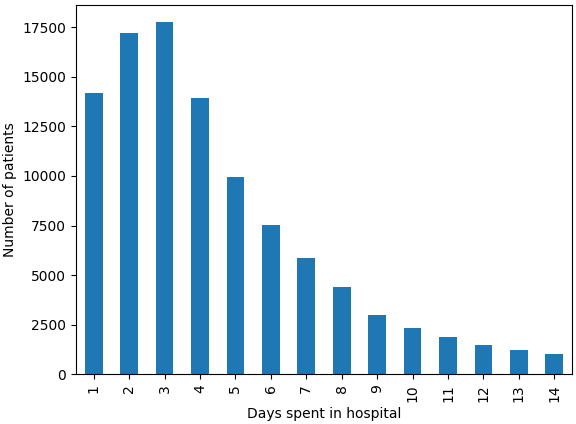
\includegraphics[width=1\textwidth]{tih_hist.png}
	\caption{Days spent in hospital per patient}
	\end{minipage}
	\hfill
	\begin{minipage}[b]{.5\textwidth}
	\centering
	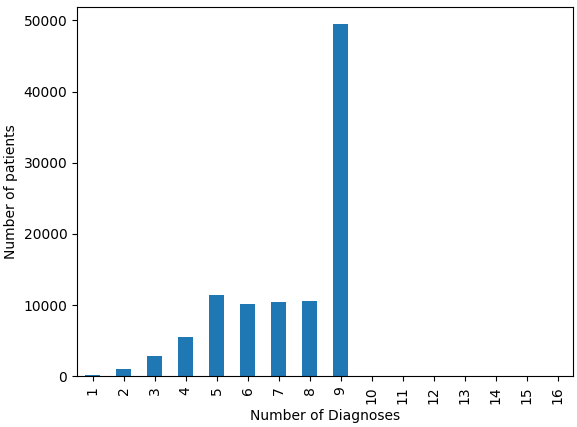
\includegraphics[width=1\textwidth]{nod_bar.png}
\caption{Diagnoses per patient}
\end{minipage}
\end{figure}

\noindent
From Figure 1 we can observe that most patients stay in the hospital between 1 and 4 days, from this we can also see that there is positive skewness. Furthermore, from Figure 2 we can observe that most patients have 9 diagnoses (almost 50\% of patients), however there are many patients that have less than 9 and rarely any patients that exceed 9 number of diagnoses. This shows that most patients had 9 diagnoses which may include diseases, injuries or any other symptom that was entered onto the system \cite{table2}. We can also make a confident assertion that a higher number of diagnoses will result in higher chance of a patient being readmitted to the hospital due to the nature of these diagnoses. It may directly correlate to the probability of readmissions.

\clearpage
\linespace
At a basic level we can visualise the distribution of diabetic patients by race and gender, the results of this can be seen below.

\begin{figure}[ht]
	\begin{minipage}[b]{.4\textwidth}
	\centering
	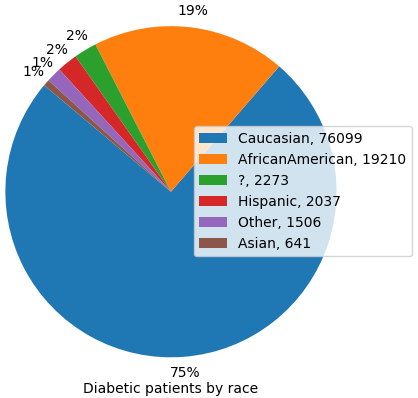
\includegraphics[width=1\textwidth]{race_pie.png}
	\caption{Proportion of diabetics by race}
	\end{minipage}
	\hfill
	\begin{minipage}[b]{.4\textwidth}
	\centering
	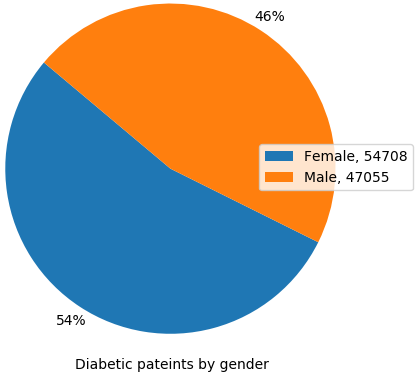
\includegraphics[width=1\textwidth]{gender_pie.png}
\caption{Proportion of diabetics by gender}
\end{minipage}
\end{figure}

\linespace
From this we can see that majority of diabetic patients admitted to US hospitals from 1999 to 2008 are mostly Caucasian (75\%). By analysing the gender split, it's almost an equal split however a higher percentage of females (54\%) than males (46\%). By looking at the ethnicity and gender features, we can confidently make the assertion that it does \textbf{not} motivate whether or not a patient is likely to be readmitted to the hospital. It does not provide us with any information as to whether a Caucasian male is more likely to be readmitted for diabetes than an African America female, for example. Thus, it may not be productive to consider these features in our model for predicting if a patient will be readmitted. 

\linespace
In the dataset there is some confusion between the type of readmission, where values are either ``NO'' ``\texttt{<30}'' or ``\texttt{>30}''. To avoid this confusion we can simply say that any value which is not ``NO'' is ``YES'' as we don't require any other information to make predictions. We can further observe the admission type of a patient and whether they have been readmitted to a hospital. Below the figures show the proportion of readmitted patients in the dataset and also the admission distribution.

\begin{figure}[ht]
	\begin{minipage}[b]{.4\textwidth}
	\centering
	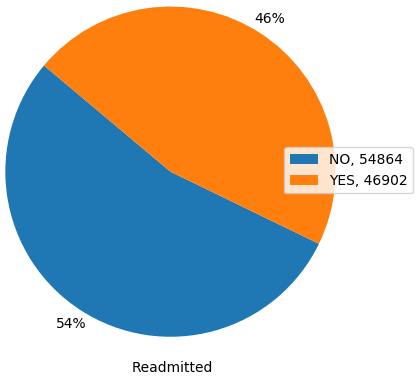
\includegraphics[width=1\textwidth]{readmitted_pie.png}
	\caption{Proportion of diabetics by race}
	\end{minipage}
	\hfill
	\begin{minipage}[b]{.4\textwidth}
	\centering
	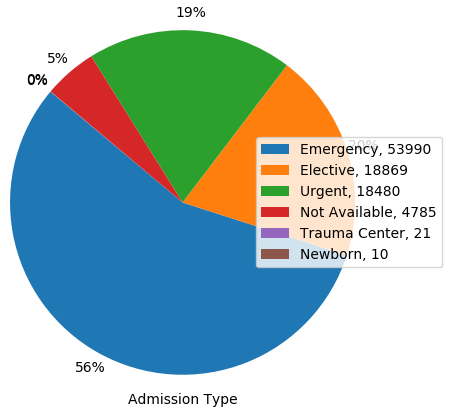
\includegraphics[width=1\textwidth]{admission_type_pie.png}
\caption{Proportion of diabetics by gender}
\end{minipage}
\end{figure}

\clearpage
From this we can see that \textit{about} half of the patients are readmitted to the hospital and in most cases the reason for the admission is Emergency. From this we can group the data and extract the following information:

\begin{table}[!ht]
    %\caption{}
    \begin{minipage}[t]{.5\linewidth}
      \caption{Readmission grouped by type of admission}
      \centering
        \begin{tabular}{|c|c|c|}
\hline
\multirow{2}{*}{Elective}      & YES & 7707  \\ 
                               & NO  & 11162 \\ \hline
\multirow{2}{*}{Emergency}     & YES & 25530 \\
                               & NO  & 28460 \\ \hline 
\multirow{2}{*}{Newborn}       & YES & 3     \\
                               & NO  & 7     \\ \hline
\multirow{2}{*}{Not Available} & YES & 2216  \\
                               & NO  & 2569  \\ \hline 
\multirow{2}{*}{Trauma Center} & YES & 0     \\
                               & NO  & 21    \\ \hline
\multirow{2}{*}{Urgent}        & YES & 8518  \\
                               & NO  & 9962  \\ \hline
\end{tabular}
    \end{minipage}%
    \begin{minipage}[t]{.5\linewidth}
      \centering
        \caption{Readmission grouped by type of age}
        \begin{tabular}{|c|c|c|}
\hline
\multirow{2}{*}{[0-10)}        & YES & 29    \\ 
                               & NO  & 132   \\ \hline
\multirow{2}{*}{[10-20)}       & YES & 264   \\
                               & NO  & 427   \\ \hline 
\multirow{2}{*}{[20-30)}       & YES & 3746 \\
                               & NO  & 911   \\ \hline
\multirow{2}{*}{[30-40)}       & YES & 1611  \\
                               & NO  & 2164  \\ \hline 
\multirow{2}{*}{[40-50)}       & YES & 4305     \\
                               & NO  & 5380    \\ \hline
\multirow{2}{*}{[50-60)}       & YES & 7585  \\
                               & NO  & 9671  \\ \hline
\multirow{2}{*}{[60-70)}       & YES & 10399  \\
                               & NO  & 12084  \\ \hline
\multirow{2}{*}{[70-80)}       & YES & 12544  \\
                               & NO  & 13524  \\ \hline
\multirow{2}{*}{[80-90)}       & YES & 8301  \\
                               & NO  & 12544  \\ \hline
\multirow{2}{*}{[90-100)}      & YES & 1118  \\
                               & NO  & 1675  \\ \hline
\end{tabular}
    \end{minipage} 
\end{table}

\noindent
In Table 1 we can notice that a lot of the patients that are admitted are admitted for ``Emergency'', and some as ``Elective'' which means that the doctors reserve a bed for the patient to be admitted for any cause. We can also see that almost 50\% of patients who are admitted for ``Emergency'' are readmitted at some point. From this we can confidently assert that the type of admission may be very important in predicting whether a patient is likely to be readmitted at some point. The same assertion can be made about age, we can see that in regards to age-group, patients that are older are admitted more frequently and this increases the chance of them being readmitted at some point. However we can also notice that patients in the age group of \texttt{[20-30)} are very likely to be readmitted, as the dataset suggests. We can also say that older people are more likely to be diabetic, thus have a higher chance of being readmitted.



  \begin{thebibliography}{1}

  \bibitem{table2} Beata Strack, Jonathan P. DeShazo, Chris Gennings, et al., “Impact of HbA1c Measurement on Hospital Readmission Rates: Analysis of 70,000 Clinical Database Patient Records,” BioMed Research International, vol. 2014, Article ID 781670, 11 pages, 2014. doi:10.1155/2014/781670 - \url{https://www.hindawi.com/journals/bmri/2014/781670/} - Table found at: \url{https://www.hindawi.com/journals/bmri/2014/781670/tab2/}

  \end{thebibliography}

\end{document}